\section{Part 2: Multidimensional (Multivariate) Kalman Filter}

\begin{frame}
   \frametitle{Part 2: Multidimensional (Multivariate) Kalman Filter}
		
		\textbf{Objectives}
				
		\begin{itemize}
			\item Kalman Filter with matrix notation for designing a multivariate Kalman Filter
            \item Linear Kalman Filter (LKF): assumes that the system dynamics are linear
			\item Mathematical derivation of Kalman Filter equations, dynamic systems modeling, and two numerical examples
		\end{itemize}
		
		\vspace{10pt}
		
		% \begin{exampleblock}{}
  % {\small ``The road to learning by precept is long, by example short and effective.''}
  % \vskip3mm
  % \hspace*\fill{\small--- Lucius Seneca}
% \end{exampleblock}


% 		\begin{framed}
% 		\begin{center}
% 		\textbf{Designing reliable systems with guaranteed performance under time dependent varying wireless channel chracteristics }
% 		\end{center}
% 		\end{framed}
\end{frame}


\subsection{Introduction}
\begin{frame}{Introduction}
\begin{columns}
    \column{0.5\textwidth} 
        \begin{itemize}
            \item Until now, we have been looking at 1D processes, like estimating the liquid temperature.
            \item But many dynamic processes have 2, 3, or even more dimensions.
            \item \textbf{Ex1:} The state vector that describes the airplane's position in space is 3D:
            \begin{equation*}
            \centering
            \begin{bmatrix}
            x\\
            y\\
            z\\
            \end{bmatrix}
            \end{equation*}
            \item \textbf{Ex2:} The state vector that describes the airplane position and velocity is 6-D:
            \begin{equation*}
            \centering
            \begin{bmatrix}
            x\\
            y\\
            z\\
            \dot{x}\\
            \dot{y}\\
            \dot{z}\\
            \end{bmatrix}
            \end{equation*}
        \end{itemize}
    \column{0.5\textwidth} 
    \begin{itemize}
        \item \textbf{Ex3:} The state vector that describes the airplane position, velocity, and acceleration is nine-dimensional:
            \begin{equation*}
            \centering
            \begin{bmatrix}
            x\\
            y\\
            z\\
            \dot{x}\\
            \dot{y}\\
            \dot{z}\\
            \ddot{x}\\
            \ddot{y}\\
            \ddot{z}\\
            \end{bmatrix}
            \end{equation*}
        
        \begin{figure}
            \centering
            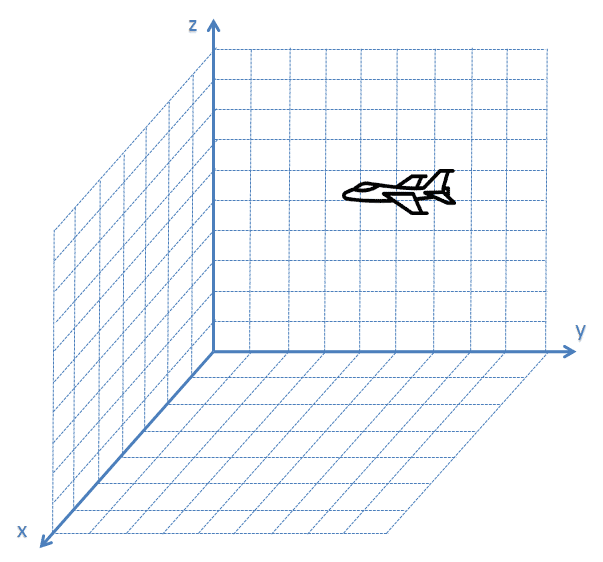
\includegraphics[width=0.5\textwidth]{Figures/Chapter2/3Dfighter.png}
            \label{fig:3Dfighter}
            \vspace{-5pt}
        \end{figure}
    \end{itemize}
\end{columns}
\end{frame}
%-------------------------------------------------
\begin{frame}{Introduction}
    % \begin{columns}
        % \column{0.5\textwidth}
    \begin{itemize}
        
    \item Assuming a constant acceleration dynamic model, we can describe the extrapolated airplane state at time $n$ by nine motion equations:
        
    \begin{align*}
     x_n = & x_{n-1} + \dot{x}_{n-1} \Delta t + \frac{1}{2}\ddot{x}_{n-1}\Delta t^2\\\nonumber
     y_n = & y_{n-1} + \dot{y}_{n-1} \Delta t + \frac{1}{2}\ddot{y}_{n-1}\Delta t^2\\\nonumber
     z_n = & z_{n-1} + \dot{z}_{n-1} \Delta t + \frac{1}{2}\ddot{z}_{n-1}\Delta t^2\\\nonumber
     \dot{x}_n = & \dot{x}_{n-1} + \ddot{x}_{n-1} \Delta t\\\nonumber
     \dot{y}_n = & \dot{y}_{n-1} + \ddot{y}_{n-1} \Delta t\\\nonumber
     \dot{z}_n = & \dot{z}_{n-1} + \ddot{z}_{n-1} \Delta t\\\nonumber
     \ddot{x}_{n} = & \ddot{x}_{n-1}\\\nonumber
     \ddot{y}_{n} = & \ddot{y}_{n-1}\\\nonumber
     \ddot{z}_{n} = & \ddot{z}_{n-1}\\\nonumber
    \end{align*}
        % \column{0.5\textwidth}
    \item Common practice to describe a multidimensional process with a single equation in matrix form.
    
    \item Second, computers are highly efficient at matrix calculations. Implementing the Kalman Filter in matrix form yields faster computation run time.
    % \end{columns}
    \end{itemize}
\end{frame}

%%%%%%%%%%%%%%%%%%%%%%%%%%%%%%%%%%%%%%%%%%%%%%%%%%%%%%%%%%%%%%%%%%%%%%%%%%%%%%%%%%%%%%%%%%%%%%%%%%%%%%%%%%%%%%%%%%%%%%%%%%%
%-------------------------------------------------
\subsection{Essential Background II}
\subsubsection{Expectation Algebra}
\begin{frame}{The Background Break - Expectation Algebra}
    % \begin{columns}
        % \column{0.5\textwidth}
        The necessary mathematical background for Kalman Filter:
            \begin{itemize}
                \item Matrix Operations: Vector/matrix addition and multiplication, transpose, Matrix inverse, Symmetric matrices
                \item Expectation Algebra
                \item Multivariate Normal Distribution (Covariance and Covariance Matrices)
            \end{itemize}
        \textbf{Expectation Algebra}
        \begin{itemize}
            \item The expectation of a random variable $X$ equal the mean of $X$: $E(X)=\mu_X$.
        \end{itemize}
         \begin{table}[]
            \centering
            \begin{tabular}{ll}
                \toprule
                \textbf{Rule} & \textbf{Notes} \\
                \toprule
                $E(X) = \mu_X = \sum x p(x)$ & $p(x)$ is PDF of $x$ \\
                $E(a) = a$ & $a$ is constant\\
                $E(aX) = aE(x)$ & $--$\\
                $E(a\pm X) = a\pm E(x)$ & $--$\\
                $E(a\pm bX) = a\pm bE(x)$ & $b$ is constant\\
                $E(X\pm Y) = E(x) \pm E(Y)$ & $Y$ is another R.V.\\
                $E(XY) = E(X)E(Y)$ & $X, Y$ are independent\\
                \bottomrule
            \end{tabular}
            \caption{Expectation Rules}
            \label{tab:ExpectationRules}
        \end{table}
        % \column{0.5\textwidth}
    % \end{columns}
\end{frame}

%-------------------------------------------------

\begin{frame}{The Background Break - Expectation Algebra}
    % \begin{columns}
        % \column{0.5\textwidth}
        The following table includes the variance and covariance expectation rules.
        \begin{itemize}
            \item Variance of a R.V. $X$: $V(X) = E\left((X-\mu_X)^2\right)$
            \item Covariance of R.V. $X$ and $Y$: $COV(X,Y) = E\left((X-\mu_X)(Y-\mu_Y)\right)$
        \end{itemize}
         \begin{table}[]
            \centering
            \begin{tabular}{ll}
                \toprule
                \textbf{Rule} & \textbf{Notes} \\
                \toprule
                $V(a) = 0$ & Variance of a constant $a$\\[0.7em]
                $V(a\pm X) = V(X)$ & Variance of $X$\\[0.7em]
                $V(X) = E(X^2) - \mu_X^2$ & $--$\\[0.7em]
                $V(a\pm X) = a^2 V(X)$ & $a$ is constant\\[0.7em]
                $COV(X,Y) =E(XY) + \mu_X \mu_Y$ & Covariance of $X$ and $Y$\\[0.7em]
                $COV(X,Y) = 0$ & If $X$ and $Y$ are Independent\\[0.7em]
                $V(X\pm Y) = V(X) + V(Y) \pm 2COV(X,Y)$ & \\[0.7em]
                $V(XY) \neq V(X) V(Y)$ & \\[0.7em]
                \bottomrule
            \end{tabular}
            \caption{Variance and Covariance Expectation Rules}
            \label{tab:Var_CoVar_Rules}
        \end{table}
\end{frame}

%-------------------------------------------------
\begin{frame}{The Background Break - Multivariate Normal Distribution}
\begin{itemize}
\item Introduction to the Kalman Filter: 
    \begin{itemize}
        \item The Kalman Filter output is a random variable.
        \item The mean of the random variable is the state estimate.
        \item The variance represents the estimation uncertainty.
        \item It provides us with the estimate and the level of confidence of its estimate.
    \end{itemize}
\item One-dimensional Kalman Filter equations include four uncertainty variables:
    \begin{enumerate}
        \item \(p_{n,n}\) is the variance of an estimate (the current state).
        \item \(p_{n+1,n}\) is the variance of a prediction (the next state).
        \item \(r_n\) is the measurement variance.
        \item \(q\) is the process noise.
    \end{enumerate}

\item Multivariate Kalman Filter
    \begin{itemize}
        \item Describes the system state by a vector with more than one variable.
        \item For example, object’s position on the plane: \[x = \begin{bmatrix} x \\ y \end{bmatrix}\] 
        \item The Kalman Filter output is a multivariate random variable.
        \item A covariance matrix describes the squared uncertainty of the multivariate random variable.
    \end{itemize}

\item Uncertainty variables of multivariate Kalman Filter
    \begin{itemize}
        \item The uncertainty variables are represented by covariance matrices:
        \begin{enumerate}
            \item \(P_{n,n}\) describes the squared uncertainty of an estimate.
            \item \(P_{n+1,n}\) describes the squared uncertainty of a prediction.
            \item \(R_n\) describes the squared measurement uncertainty.
            \item \(Q\) describes the process noise.
        \end{enumerate}
    \end{itemize}
\end{itemize}    
\end{frame}
%-------------------------------------------------
\subsubsection{Covariance}
\begin{frame}{The Background Break - Multivariate Normal Distribution}
    \begin{itemize}
        \item Covariance is a measure of the strength of the correlation between two or more sets of random variates.
        \item On the x-y plane, variance in measurements exists due to random error.
    \end{itemize}
        \begin{itemize}
            \item \textbf{Uncorrelated measurements:}
            \begin{itemize}
                \item The x and y values don't depend on each other. The covariance of x and y equals zero.
                \item For the blue data set, a circular distribution shape indicates equal variance.
                \item For the red data set, an elliptic distribution shape indicates greater variance in x values.
            \end{itemize}
            \item \textbf{Correlated measurements:}
            \begin{itemize}
                \item Dependency exists between x and y values.
                \item For the green data set, positive correlation and covariance due to concurrent increase.
                \item For the cyan data set, negative correlation and covariance due to inverse changes.
            \end{itemize}
        \end{itemize}
    \begin{figure}
        \centering
    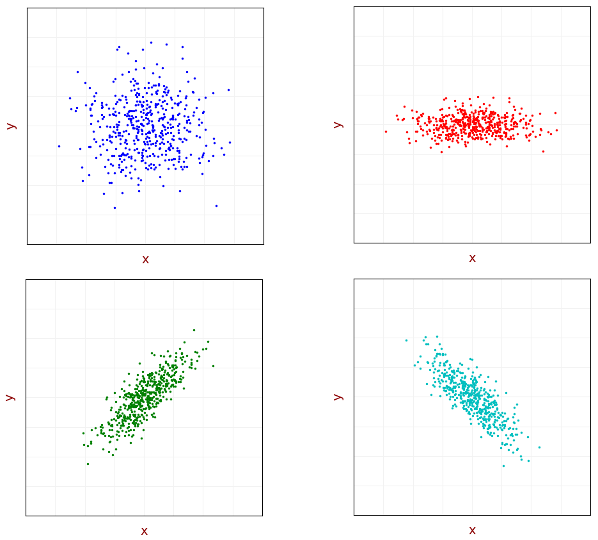
\includegraphics[width=0.4\textwidth]{Figures/Background2/CovarianceIllustration.png}
        \caption{Examples of different measurement sets.}
    \end{figure}

\end{frame}
%--------------------------------------------------------------------
\begin{frame}{The Background Break - Covariance}
The covariance between population $X$ and population $Y$ with size $N$
    \begin{align}
       \text{COV} (X, Y) & = \frac{1}{N} \sum_{i=1}^{N} (x_i - \mu_x)(y_i - \mu_y)\nonumber\\ & = \frac{1}{N} \sum_{i=1}^{N} (x_i y_i) - \mu_x \mu_y \nonumber
    \end{align}
The covariance of a sample with size $N$ is normalized by $N - 1$
    \begin{align}
     \text{COV} (X, Y) & = \frac{1}{N - 1} \sum_{i=1}^{N} (x_i - \mu_x)(y_i - \mu_y)\nonumber \\ &= \frac{1}{N - 1} \left( \sum_{i=1}^{N} x_i y_i \right) - \frac{N}{N - 1} \mu_x \mu_y \nonumber\\
     & = \frac{1}{N - 1}{\mathbf{x}^T y - \frac{N}{N - 1} \mu_x \mu_y}\nonumber \quad [\text{In vector notation}]\\
     & = \frac{1}{N - 1}\mathbf{x}^T y \quad [\text{For a zero-mean random variable}]\nonumber
     \end{align}
\end{frame}

%-------------------------------------------------
\subsubsection{Covariance Matrix}
\begin{frame}{The Background Break - Covariance Matrix}
A covariance matrix is a square matrix that represents the covariance between each
pair of elements in a given multivariate random variable.

For a two-dimensional random variable, the covariance matrix is given by
\begin{equation*}
    \Sigma = 
    \begin{bmatrix}
        \sigma_{xx} & \sigma_{xy} \\
        \sigma_{yx} & \sigma_{yy}
    \end{bmatrix}
    =
    \begin{bmatrix}
        \sigma^2_{x} & \sigma_{xy} \\
        \sigma_{yx} & \sigma^2_{y}
    \end{bmatrix}
    =
    \begin{bmatrix}
        \text{VAR}(x) & \text{COV}(x, y) \\
        \text{COV}(y, x) & \text{VAR}(y)
    \end{bmatrix}
\end{equation*}
Note that the off-diagonal entries of the covariance matrix are equal since $\text{COV}(x, y) =
\text{COV}(y, x)$. If $x$ and $y$ are uncorrelated, the off-diagonal entries of the covariance
matrix are zero.


\textbf{Properties of the covariance matrix:}
\begin{itemize}
    \item The diagonal entries of this covariance matrix are the variances of the components of the multivariate random variable:
    $$\Sigma_{ii} = \sigma^2_{i}$$
    \item Since the diagonal entries are all non-negative, the trace (the sum of diagonal entries) of this covariance matrix is non-negative:
    $$\text{tr}(\mathbf{\Sigma}) = \sum_{i=1}^{n} \Sigma_{ii} \geq 0$$ 
    \item Since \(\Sigma_{ij} = \sigma_{ij} = \sigma_{ji} = \Sigma_{ji}\), the covariance matrix is symmetric:
    $$\mathbf{\Sigma} = \mathbf{\Sigma^T}$$
    \item The covariance matrix is \textbf{positive semidefinite}. The matrix \(\mathbf{A}\) is called positive semidefinite if \(\mathbf{v}^T \mathbf{A} \mathbf{v} \geq 0\), for any vector \(v\). \textbf{The eigenvalues of \(\mathbf{A}\) are non-negative}.
\end{itemize}

\end{frame}
%-------------------------------------------------
\subsubsection{Covariance Matrix and Expectation}
\begin{frame}{The Background Break - Expectation Algebra - Covariance Matrix and Expectation}
\begin{itemize}
    \item Assume a vector $\mathbf{x}$ with $k$ elements:
        \begin{equation*}
            \centering
            \mathbf{x}=\begin{bmatrix}
            x_1\\
            x_2\\
            \vdots\\
            x_k\\
            \end{bmatrix}
            \end{equation*}
    \item The covariance matrix of the vector $\mathbf{x}$ is:
            \begin{align*}
            \centering
            COV(\mathbf{x}) = & E\left((\mathbf{x} -\mathbf{\mu}_x)(\mathbf{x} -\mathbf{\mu}_x)^T\right)\\
            = & E\left(\begin{bmatrix}
            (x_1-\mu_{x_1})\\
            (x_2-\mu_{x_2})\\
            \vdots\\
            (x_k-\mu_{x_k})\\
            \end{bmatrix}
            \Big[(x_1-\mu_{x_1})~~(x_2-\mu_{x_2})~~\cdots~~ (x_k-\mu_{x_k})\Big]
            \right)
            \end{align*}
\end{itemize}
\end{frame}


%-------------------------------------------------------
\subsubsection{Multivariate Normal Distribution}
\begin{frame}{The Background Break - Multivariate Normal Distribution}

Univariate Gaussian distribution:
$$p(x|\mu, \sigma) = \frac{1}{\sqrt{2\pi\sigma^2}} \exp\left(-\frac{(x - \mu)^2}{2\sigma^2}\right)$$

The $n$ - dimensional multivariate normal distribution:
$$p(\mathbf{x}|\boldsymbol{\mu},\mathbf{\Sigma)} = \frac{1}{\sqrt{(2\pi)^n |\mathbf{\Sigma}|}} \exp\left(-\frac{1}{2}(\mathbf{x} - \boldsymbol{\mu})^T \mathbf{\Sigma}^{-1} (\mathbf{x} - \boldsymbol{\mu})\right)$$
\begin{itemize}
    \item $\mathbf{x}$ is an \(n\)-dimensional random vector,
    \item $\boldsymbol{\mu}$ is an \(n\)-dimensional mean vector,
    \item $\boldsymbol{\Sigma}$ is a square \(n \times n\) covariance matrix,
    \item $\boldsymbol{\Sigma}^{-1}$ is the inverse of the covariance matrix,
    \item $|\boldsymbol{\Sigma}| \equiv \det(\boldsymbol{\Sigma})$ is the determinant of ${\boldsymbol {\Sigma }}$.
\end{itemize}
\vspace{-10pt}
\begin{columns}
        \column{0.5\textwidth} 
            \begin{figure}
    \centering
    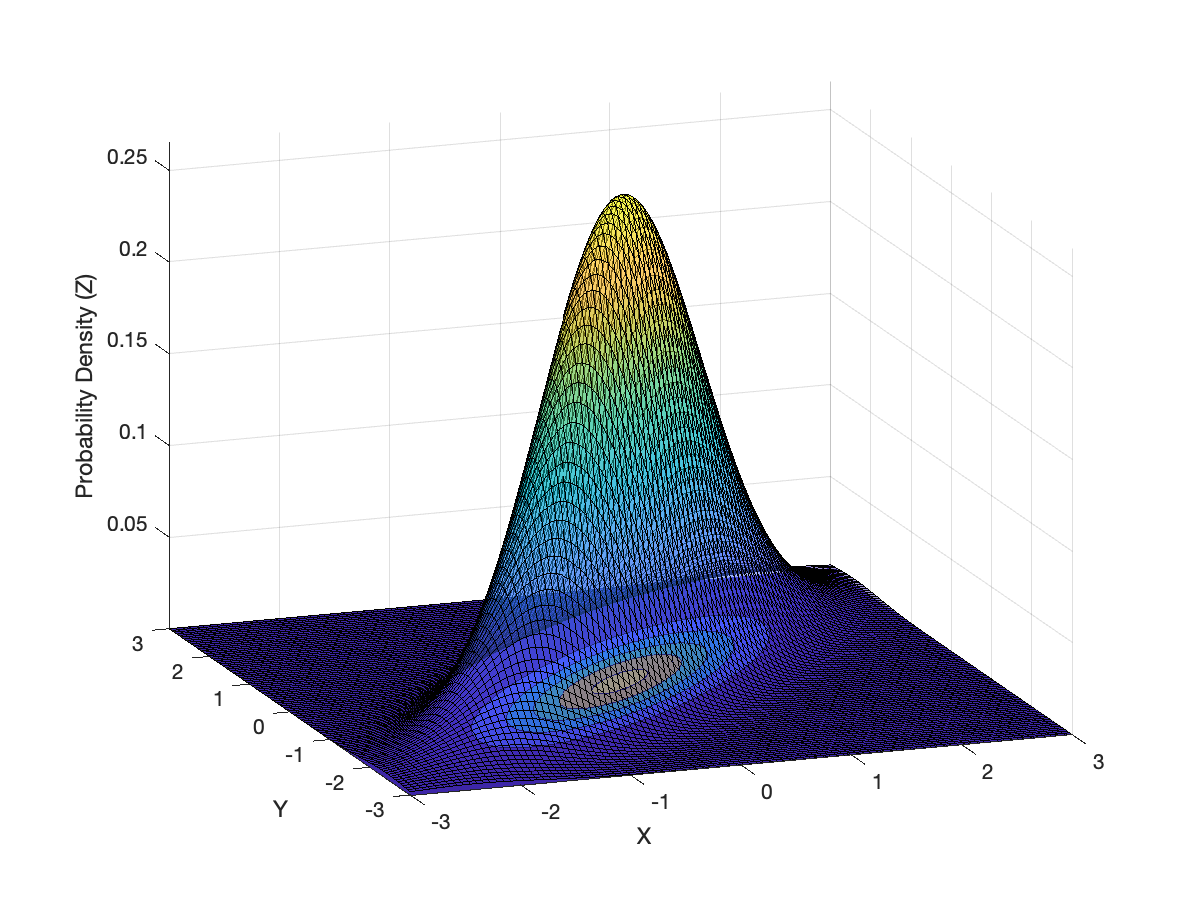
\includegraphics[width=0.75\textwidth]{Figures/Background2/GaussuanSurface_Corr_0.8.eps}
        \vspace{-10pt}
        \caption{Bivariate Gaussian distribution ($\rho=0.4$).}
    \end{figure}
        \column{0.5\textwidth}
            \begin{figure}
    \centering
    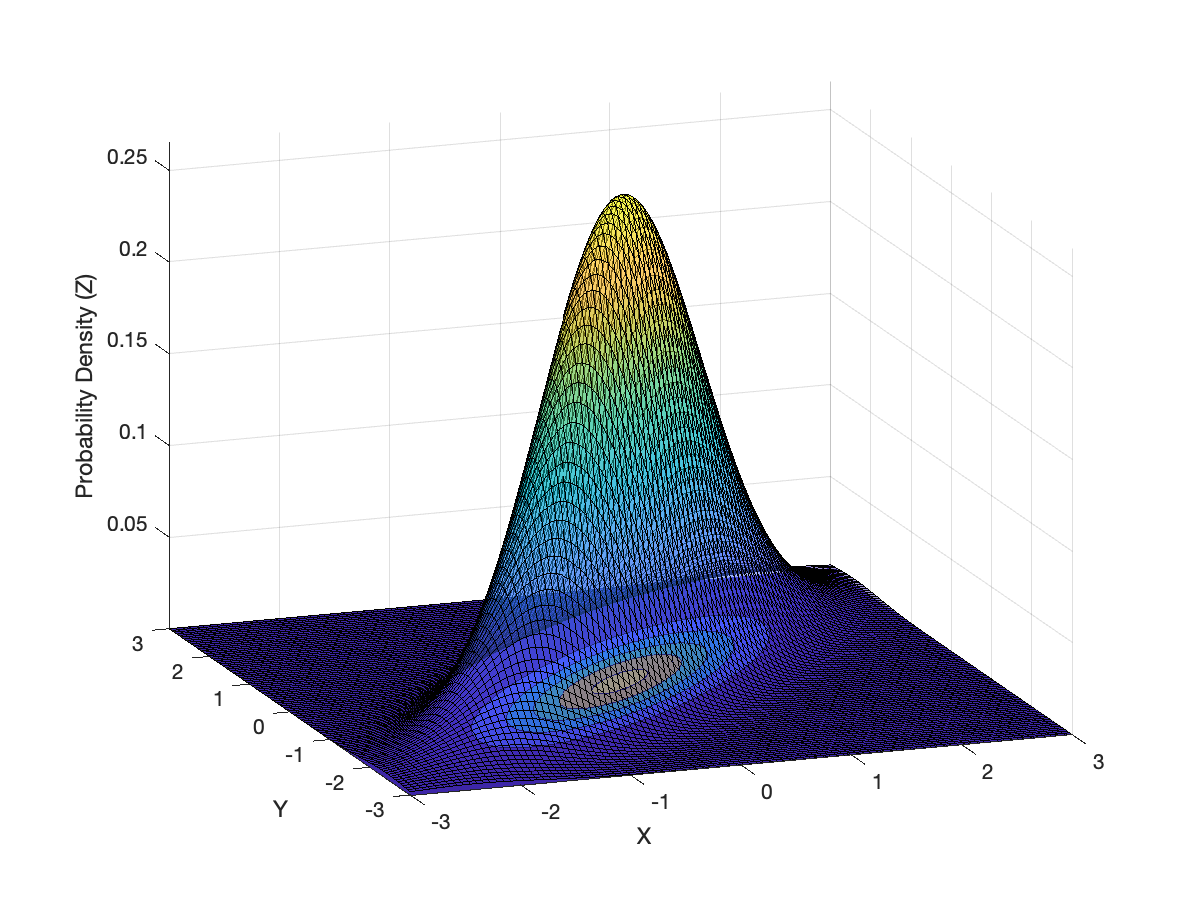
\includegraphics[width=0.75\textwidth]{Figures/Background2/GaussuanSurface_Corr_0.8.eps}
        \vspace{-10pt}
        \caption{Bivariate Gaussian distribution ($\rho=0.8$).}
    \end{figure}
\end{columns}



\end{frame}

%-------------------------------------------------------
\subsubsection{Bivariate Normal Distribution}
\begin{frame}{The Background Break - Bivariate Normal Distribution}
\begin{columns}
        \column{0.5\textwidth} 
For univariate distribution, the area between the $1\sigma$ boundaries is 68.26\% of the total area under the Gaussian function.
                \begin{figure}
            \centering
    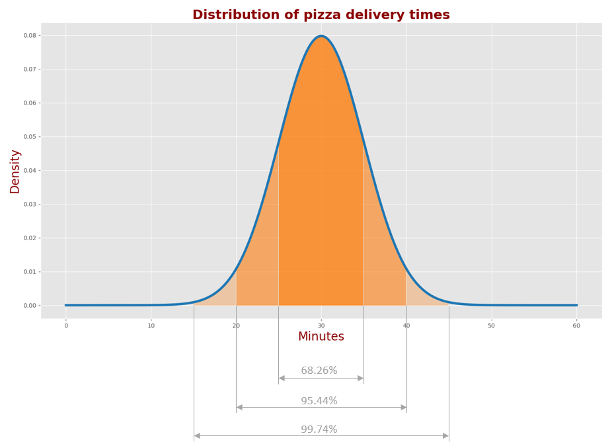
\includegraphics[width=1\textwidth]{Figures/Background2/UnivariateGaussian.png}
        \vspace{-10pt}
        \caption{Univariate Gaussian.}
    \end{figure}
        \column{0.5\textwidth}
        The probability of the bivariate normal distribution is a volume of the 3D
Gaussian function. For example, the volume of the 3D Gaussian function sliced at  $1\sigma$ 
level is 39.35\% of the total volume of the 3D Gaussian function.
        \begin{figure}
            \centering
    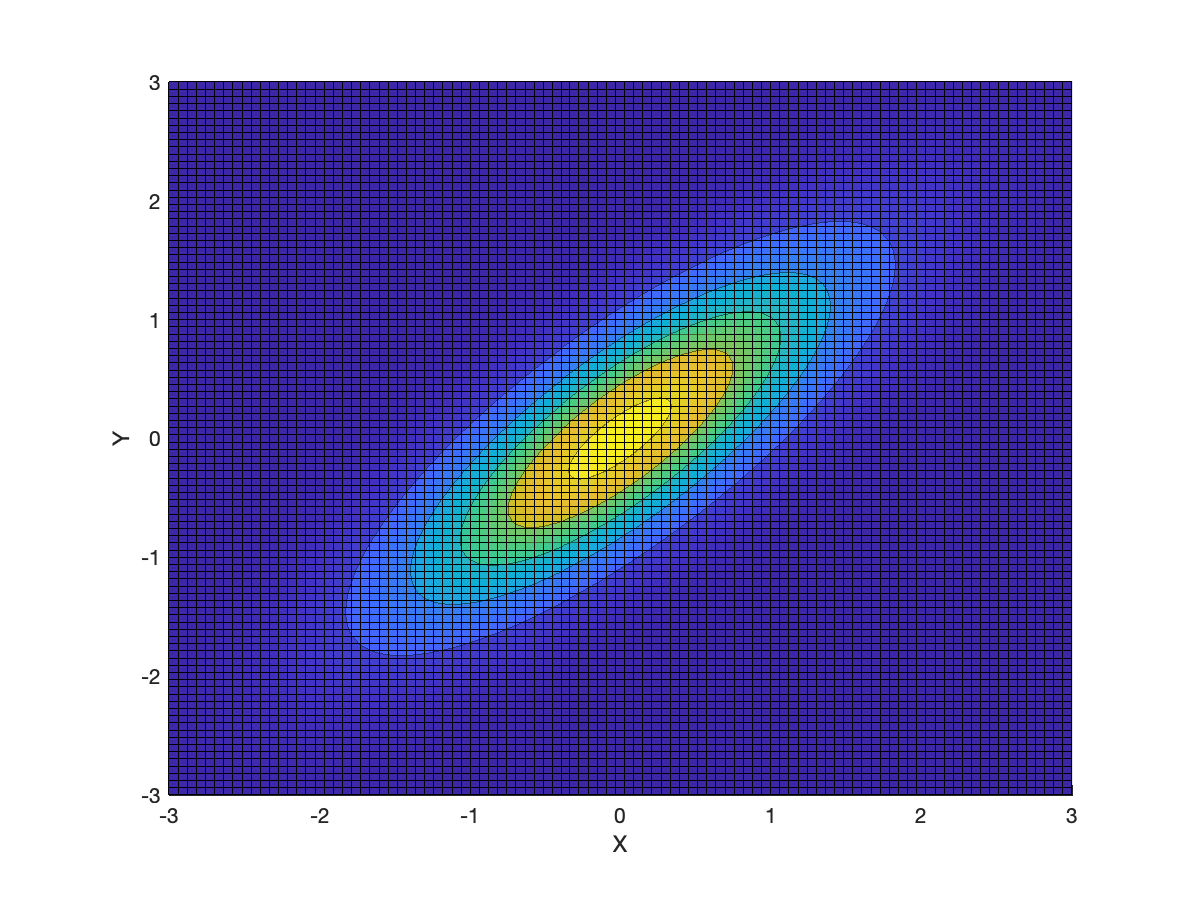
\includegraphics[width=1\textwidth]{Figures/Background2/GaussianContour_Corr_0.8.eps}
        \vspace{-10pt}
        \caption{Bivariate Gaussian distribution - Contour ($\rho=0.4$).}
    \end{figure}
    \texttt{\tiny [Code: Multivariate KF/bivariateGaussian\_withContours.m]}
\end{columns}
\end{frame}
%-------------------------------------------------------
\subsubsection{Covariance Ellipse}
\begin{frame}{The Background Break - Bivariate Normal Distribution - Covariance Ellipse}

\begin{itemize}
    \item The covariance ellipse represents an \textit{iso-contour} of the Gaussian distribution and allows visualization of a $1\sigma$ confidence interval in two dimensions. 
    \item It provides a geometric interpretation of the covariance matrix.
    \item Any ellipse can be described by four parameters:
    \begin{itemize}
        \item Ellipse center $\mu_x$, $\mu_y$
        \item Half-major axis $a$
        \item Half-minor axis $b$
        \item Orientation angle $\theta$
    \end{itemize}
    \begin{figure}
        \centering
        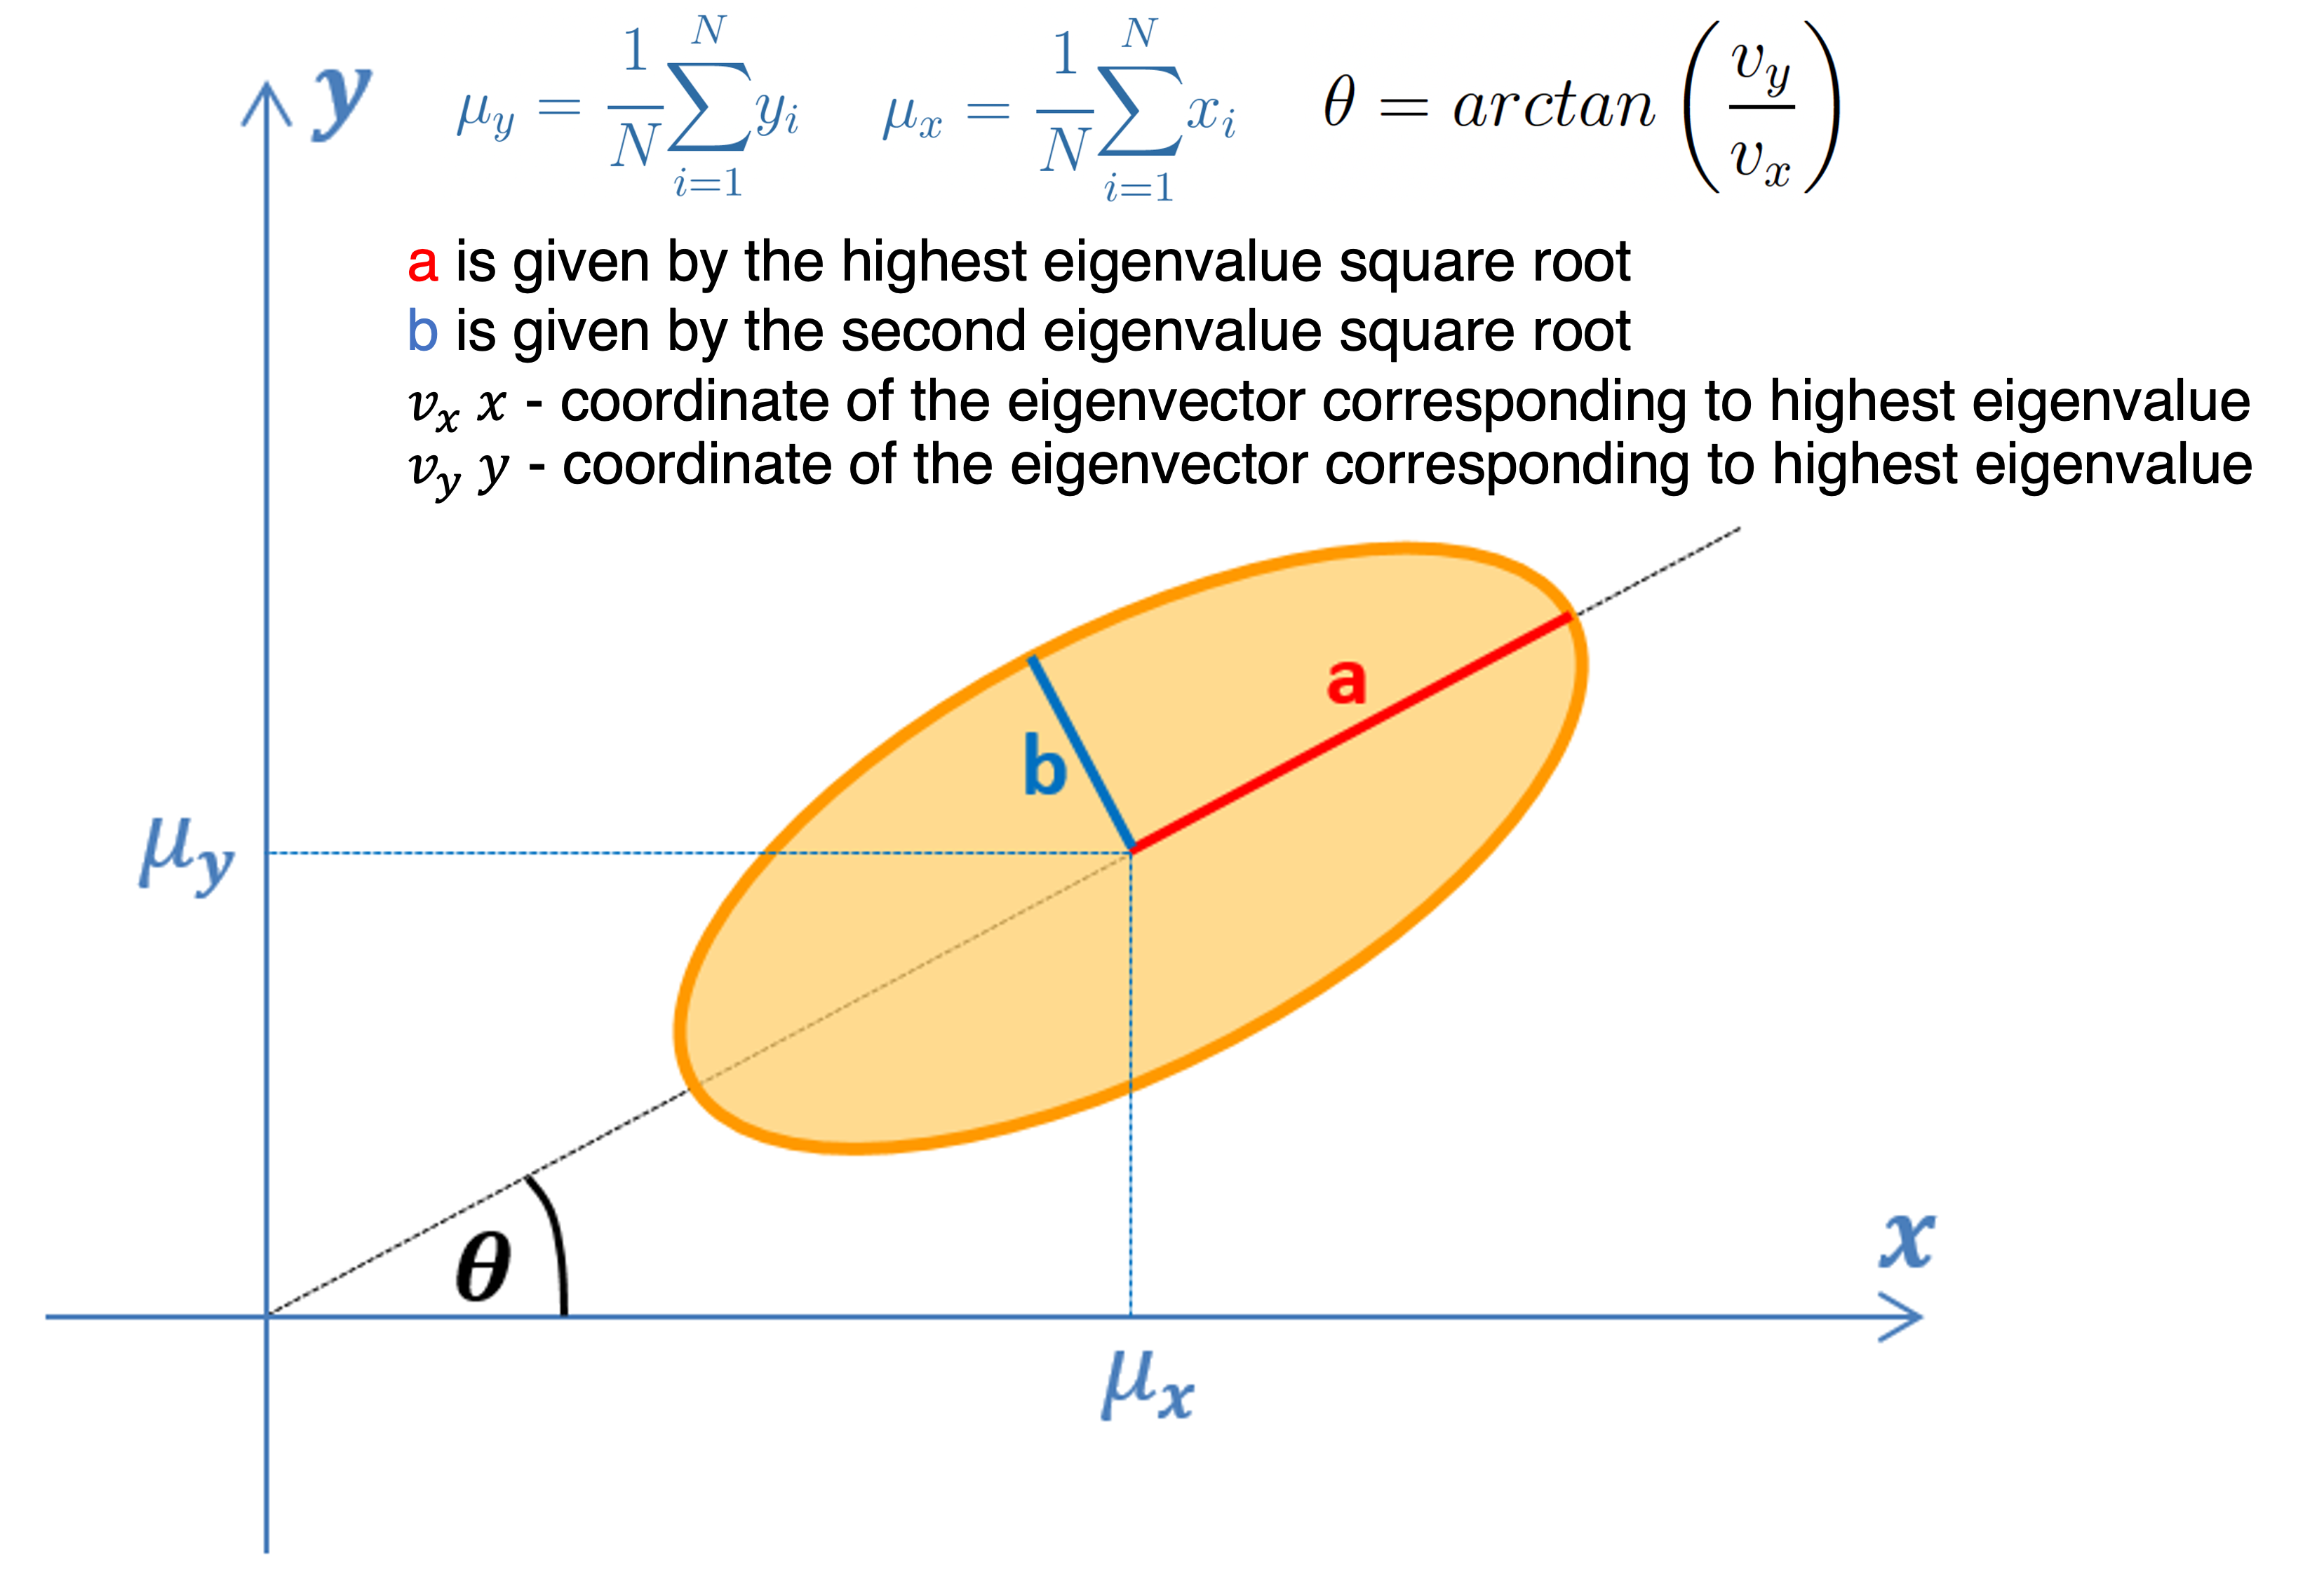
\includegraphics[width=0.6\textwidth]{Figures/Background2/CovarianceEllipse.png}
        \vspace{-10pt}
        \caption{Covariance ellipse.}
    \end{figure}
    

\end{itemize}

\end{frame}
%-------------------------------------------------------
\subsubsection{Confidence Ellipse}
\begin{frame}{The Background Break - Confidence Ellipse and Finding Probability Boundaries}

\begin{itemize}
    \item Often there is an interest in finding the boundaries of specific probability. For example, for 95\% probability, we should find the boundary that includes 95\% of Gaussian function volume.
    \item The projection of this boundary onto the \(x - y\) plane is the confidence ellipse. 
    \item \textbf{Find an elliptical scale factor \(k\), that extends the covariance ellipse to the confidence ellipse associated with 95\% probability.}
    \end{itemize}
    \begin{figure}
        \centering
        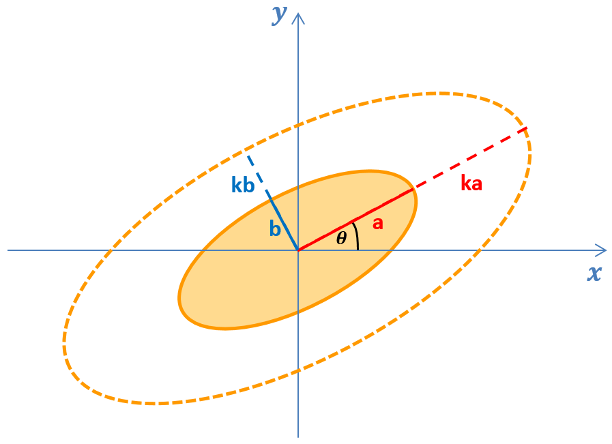
\includegraphics[width=0.6\textwidth]{Figures/Background2/ConfidenceEllipse.png}
        \vspace{-10pt}
        \caption{Covariance ellipse.}
    \end{figure}
\end{frame}
\begin{frame}{The Background Break - Confidence Ellipse and Finding Probability Boundaries}
   \begin{itemize} 
    \item As \(\sigma_x\) and \(\sigma_y\) represent the standard deviations of stochastically independent random variables, the addition theorem for the chi-square distribution may be used to show that the probability associated with a confidence ellipse is given by:
    $$p = 1 - \exp\left(-\frac{1}{2}k^2\right)$$
    \item For a covariance ellipse \(k = 1\), the probability associated with a covariance ellipse is:
    $$p = 1 - \exp\left(-\frac{1}{2}\right) = 39.35\%$$
    \item For a given probability, we can find an elliptical scale factor: $$k = \sqrt{-2\ln(1 - p)}$$
    \item For the probability of 95\%: $$k = \sqrt{-2\ln(1 - 0.95)} = 2.45$$
\end{itemize}

The properties of the confidence ellipse associated with 95\% probability are:
\begin{itemize}
    \item Ellipse center \((\mu_x, \mu_y)\) is similar to the covariance ellipse.
    \item Orientation angle \(\theta\) is similar to the covariance ellipse.
    \item Half-major axis length is \(2.45a\) – a scaled half-major axis of the covariance ellipse.
    \item Half-minor axis length is \(2.45b\) – a scaled half-minor axis of the covariance ellipse.
\end{itemize}
\end{frame}

%%%%%%%%%%%%%%%%%%%%%%%%%%%%%%%%%%%%%%%%%%%%%%%%%%%%%%%%%%%%%%%%%%%%%%%%%%%%%%%%%%%%%%%%%%%%%%%%%%%%%%%%%%%%%%%%%%%%%%%%%%%

\subsection{State Extrapolation Equation}
\begin{frame}{State Extrapolation Equation or Predictor Equation or Transition Equation or Dynamic Model or State Space Model}
Using the \textcolor{blue}{state extrapolation equation}, we can predict the \textbf{next system state} based
on the knowledge of the \textbf{current state}. \textcolor{blue}{It extrapolates the state vector from the
present (time step $n$) to the future (time step $n + 1$).}   

The State Extrapolation Equation can be expressed as:
\begin{minipage}{1\linewidth} % Adjust the width as needed
\begin{exampleblock}{}{
\begin{equation}
\mathbf{\hat{x}}_{n+1,n} = \mathbf{F} \mathbf{\hat{x}}_{n,n} + \mathbf{G} \mathbf{u}_{n} + \mathbf{w}_{n}\tag{1}
\end{equation}

where:
\begin{itemize}
    \item $\mathbf{\hat{x}}_{n+1,n}$ is a predicted system state vector at time step $n + 1$.
    \item $\mathbf{\hat{x}}_{n,n}$ is an estimated system state vector at time step $n$.
    \item $\mathbf{u}_{n}$ is a control variable or input variable - a measurable (deterministic) input to the system.
    \item $\mathbf{w}_{n}$ is a process noise or disturbance - an unmeasurable input that affects the state.
    \item $\mathbf{F}$ is a state transition matrix.
    \item $\mathbf{G}$ is a control matrix or input transition matrix (mapping control to state variables).
\end{itemize}}
\end{exampleblock}
\end{minipage}

\textit{*The process noise $w_n$ does not typically appear directly in the equations of
interest. Instead, this term is used to model the uncertainty in the Covariance
Extrapolation Equation.}
\end{frame}
%--------------------------------------------------

\begin{frame}{State Extrapolation Equation}
\begin{itemize}
    \item The state variables may represent attributes of the system that we wish to know. For example, a moving vehicle has three attributes: position, velocity, and acceleration.
\begin{figure}
    \centering
    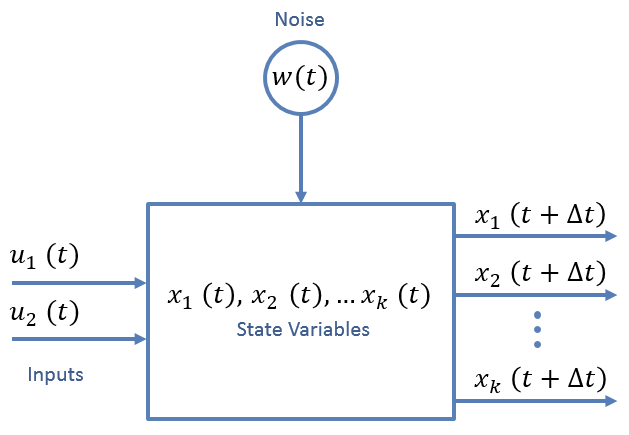
\includegraphics[width=0.5\linewidth]{Figures//Chapter2/KalmanFilterExtrapolation.png}
    \caption{Kalman Filter Extrapolation}
    \label{fig:KF_Extrapolation}
\end{figure}
\end{itemize}
\end{frame}
%---------------------------------------
\begin{frame}{State Extrapolation Equation}
Which attributes are the state variables, and which attributes are the input to the system?
\begin{itemize}
    \item Moving mechanical systems have attributes such as position, velocity, acceleration, and drag.
    \item A force that acts on a system should be considered an external forcing function, i.e., an input to the system that controls the state vector (position and velocity in the constant acceleration case).
    \item Newton’s second law tells us that $F = ma$. Thus we can consider acceleration as an external input to the system.
    \item The position and the velocity are the primary state variables of interest.
\end{itemize}

\begin{columns}
        \column{0.5\textwidth} 
        \textcolor{blue}{In a spring system, the force applied to the spring $F(t)$ is an input $u(t)$, while the spring displacement $x(t)$ is the system state.}
        \begin{figure}
            \centering
            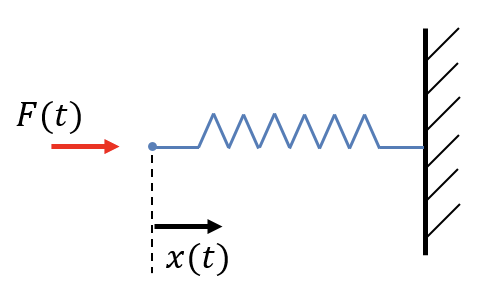
\includegraphics[width=0.7\textwidth]{Figures//Chapter2/SpringSystem.png}
            \caption{Spring System}
            \label{fig:SpringSystem}
        \end{figure}
        
        \column{0.5\textwidth}
        \textcolor{blue}{For a falling object, the inputs are the gravitational force $F_g$ and the drag force $F_{\text{drag}}(t)$, while the object height $h(t)$ and velocity $v(t)$ are the system states.}
        \begin{figure}
            \centering
            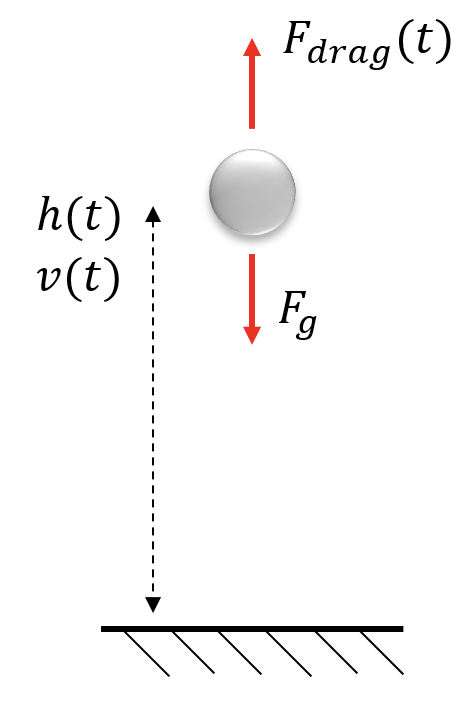
\includegraphics[width=0.3\textwidth]{Figures//Chapter2/FallingObject.png}
            \vspace{-10pt}
            \caption{Falling Object}
            \label{fig:FallingObject}
        \end{figure}
\end{columns}

\end{frame}    

%--------------------------------------------------
\subsection{Example - airplane - no control input}
\begin{frame}{State Extrapolation Equation (Example - airplane - no control input)}
Let's define the State Extrapolation Equation for an airplane moving in three-dimensional space with constant acceleration (i.e., there is no control input, $u_n = 0$).

The state vector $\mathbf{\hat{x}}_n$ ( describing the estimated airplane position, velocity, and acceleration in a cartesian coordinate system $(x, y, z)$), the state transition matrix $\mathbf{F}$ is:
\begin{columns}
        \column{0.2\textwidth} 
           \begin{equation*}
            \centering
            \mathbf{\hat{x}}_n =
            \begin{bmatrix}
            \hat{x}_n\\
            \hat{y}_n\\
            \hat{z}_n\\
            \hat{\dot{x}}_n\\
            \hat{\dot{y}}_n\\
            \hat{\dot{z}}_n\\
            \hat{\ddot{x}}_n\\
            \hat{\ddot{y}}_n\\
            \hat{\ddot{z}}_n\\
            \end{bmatrix}
            \end{equation*}
        \column{0.8\textwidth}
            $$\mathbf{F} =
\begin{bmatrix}
1 & 0 & 0 & \Delta t & 0 & 0 & 0.5\Delta t^2 & 0 & 0 \\
0 & 1 & 0 & 0 & \Delta t & 0 & 0 & 0.5\Delta t^2 & 0 \\
0 & 0 & 1 & 0 & 0 & \Delta t & 0 & 0 & 0.5\Delta t^2 \\
0 & 0 & 0 & 1 & 0 & 0 & \Delta t & 0 & 0 \\
0 & 0 & 0 & 0 & 1 & 0 & 0 & \Delta t & 0 \\
0 & 0 & 0 & 0 & 0 & 1 & 0 & 0 & \Delta t \\
0 & 0 & 0 & 0 & 0 & 0 & 1 & 0 & 0 \\
0 & 0 & 0 & 0 & 0 & 0 & 0 & 1 & 0 \\
0 & 0 & 0 & 0 & 0 & 0 & 0 & 0 & 1 \\
\end{bmatrix}$$ 
\end{columns}

$$\quad\quad\begin{bmatrix}
\hat{x}_{n+1,n} \\
\hat{y}_{n+1,n} \\
\hat{z}_{n+1,n} \\
\dot{\hat{x}}_{n+1,n} \\
\dot{\hat{y}}_{n+1,n} \\
\dot{\hat{z}}_{n+1,n} \\
\ddot{\hat{x}}_{n+1,n} \\
\ddot{\hat{y}}_{n+1,n} \\
\ddot{\hat{z}}_{n+1,n}
\end{bmatrix}
=
\begin{bmatrix}
1 & 0 & 0 & \Delta t & 0 & 0 & 0.5\Delta t^2 & 0 & 0 \\
0 & 1 & 0 & 0 & \Delta t & 0 & 0 & 0.5\Delta t^2 & 0 \\
0 & 0 & 1 & 0 & 0 & \Delta t & 0 & 0 & 0.5\Delta t^2 \\
0 & 0 & 0 & 1 & 0 & 0 & \Delta t & 0 & 0 \\
0 & 0 & 0 & 0 & 1 & 0 & 0 & \Delta t & 0 \\
0 & 0 & 0 & 0 & 0 & 1 & 0 & 0 & \Delta t \\
0 & 0 & 0 & 0 & 0 & 0 & 1 & 0 & 0 \\
0 & 0 & 0 & 0 & 0 & 0 & 0 & 1 & 0 \\
0 & 0 & 0 & 0 & 0 & 0 & 0 & 0 & 1
\end{bmatrix}
\begin{bmatrix}
\hat{x}_{n,n} \\
\hat{y}_{n,n} \\
\hat{z}_{n,n} \\
\dot{\hat{x}}_{n,n} \\
\dot{\hat{y}}_{n,n} \\
\dot{\hat{z}}_{n,n} \\
\ddot{\hat{x}}_{n,n} \\
\ddot{\hat{y}}_{n,n} \\
\ddot{\hat{z}}_{n,n}
\end{bmatrix}$$

       
\end{frame}
%--------------------------------------------------
\begin{frame}{State Extrapolation Equation (Example - airplane - no control input)}
The state update equations after matrix multiplication are given by:
\begin{align*}
\hat{x}_{n+1,n} &= \hat{x}_{n,n} + \hat{\dot{x}}_{n,n}\Delta t + \frac{1}{2}\hat{\ddot{x}}_{n,n}\Delta t^2 \\
\hat{y}_{n+1,n} &= \hat{y}_{n,n} + \hat{\dot{y}}_{n,n}\Delta t + \frac{1}{2}\hat{\ddot{y}}_{n,n}\Delta t^2 \\
\hat{z}_{n+1,n} &= \hat{z}_{n,n} + \hat{\dot{z}}_{n,n}\Delta t + \frac{1}{2}\hat{\ddot{z}}_{n,n}\Delta t^2 \\
\hat{\dot{x}}_{n+1,n} &= \hat{\dot{x}}_{n,n} + \hat{\ddot{x}}_{n,n}\Delta t \\
\hat{\dot{y}}_{n+1,n} &= \hat{\dot{y}}_{n,n} + \hat{\ddot{y}}_{n,n}\Delta t \\
\hat{\dot{z}}_{n+1,n} &= \hat{\dot{z}}_{n,n} + \hat{\ddot{z}}_{n,n}\Delta t \\
\hat{\ddot{x}}_{n+1,n} &= \hat{\ddot{x}}_{n,n} \\
\hat{\ddot{y}}_{n+1,n} &= \hat{\ddot{y}}_{n,n} \\
\hat{\ddot{z}}_{n+1,n} &= \hat{\ddot{z}}_{n,n}
\end{align*}
\end{frame}

%------------------------------------------------
\subsection{Example - airplane - with control input}
\begin{frame}{State Extrapolation Equation (Example - airplane - with control input)}

Considering additional information about the airplane
acceleration (based on the pilot’s controls) based on the pilot’s commands.

\begin{columns}
        \column{0.5\textwidth}
        The state vector $\mathbf{\hat{x}}_n$ ( describing the estimated airplane position and velocity a cartesian coordinate system $(x, y, z)$) is:
           \begin{equation*}
            \centering
            \mathbf{\hat{x}}_n =
            \begin{bmatrix}
            \hat{x}_n\\
            \hat{y}_n\\
            \hat{z}_n\\
            \hat{\dot{x}}_n\\
            \hat{\dot{y}}_n\\
            \hat{\dot{z}}_n\\
            \end{bmatrix}
            \end{equation*}
        The control vector $u_n$ that describes the measured airplane acceleration in a cartesian coordinate system $(x, y, z)$ is:
        \begin{equation*}
            \centering
            \mathbf{{u}}_n =
            \begin{bmatrix}
            \hat{\ddot{x}}_n\\
            \hat{\ddot{y}}_n\\
            \hat{\ddot{z}}_n\\
            \end{bmatrix}
        \end{equation*} 
        \column{0.5\textwidth}
        The state transition matrix $\mathbf{F}$ is:
        $$\mathbf{F} = \begin{bmatrix}
        1 & 0 & 0 & \Delta t & 0 & 0 \\
        0 & 1 & 0 & 0 & \Delta t & 0 \\
        0 & 0 & 1 & 0 & 0 & \Delta t\\
        0 & 0 & 0 & 1 & 0 & 0 \\
        0 & 0 & 0 & 0 & 1 & 0 \\
        0 & 0 & 0 & 0 & 0 & 1 \\
        \end{bmatrix}$$ 
        The control matrix $\mathbf{G}$ is:
        $$\mathbf{G} = \begin{bmatrix}
        0.5\Delta t^2 & 0 & 0 \\
        0 & 0.5\Delta t^2 & 0 \\
        0 & 0 & 0.5\Delta t^2 \\
        \Delta t & 0 & 0 \\
        0 & \Delta t & 0 \\
        0 & 0 & \Delta t \\
        \end{bmatrix}$$
        \end{columns}

\end{frame}
%-----------------------------------------------
%------------------------------------------------
\begin{frame}{State Extrapolation Equation (Example - airplane - with control input)}

The state extrapolation equation is:
$$\hat{x}_{n+1,n} = \mathbf{F}\hat{x}_{n,n} + \mathbf{G}u_{n,n}$$

Given the system dynamics, the state update can be expressed as:
\begin{equation}
\left[
\begin{array}{c}
\hat{x}_{n+1,n} \\
\hat{y}_{n+1,n} \\
\hat{z}_{n+1,n} \\
\dot{\hat{x}}_{n+1,n} \\
\dot{\hat{y}}_{n+1,n} \\
\dot{\hat{z}}_{n+1,n} \\
\end{array}
\right]
\!=\!
\left[
\begin{array}{cccccc}
1 & 0 & 0 & \Delta t & 0 & 0 \\
0 & 1 & 0 & 0 & \Delta t & 0 \\
0 & 0 & 1 & 0 & 0 & \Delta t \\
0 & 0 & 0 & 1 & 0 & 0 \\
0 & 0 & 0 & 0 & 1 & 0 \\
0 & 0 & 0 & 0 & 0 & 1 \\
\end{array}
\right]
\left[
\begin{array}{c}
\hat{x}_{n,n} \\
\hat{y}_{n,n} \\
\hat{z}_{n,n} \\
\dot{\hat{x}}_{n,n} \\
\dot{\hat{y}}_{n,n} \\
\dot{\hat{z}}_{n,n} \\
\end{array}
\right]
\!+\!
\left[
\begin{array}{ccc}
0.5\Delta t^2 & 0 & 0 \\
0 & 0.5\Delta t^2 & 0 \\
0 & 0 & 0.5\Delta t^2 \\
\Delta t & 0 & 0 \\
0 & \Delta t & 0 \\
0 & 0 & \Delta t \\
\end{array}
\right]
\left[
\begin{array}{c}
\ddot{x}_n \\
\ddot{y}_n \\
\ddot{z}_n \\
\end{array}
\right]\nonumber
\end{equation}

\end{frame}
%---------------------------------------------
\subsection{Example – Falling Object}
\begin{frame}{State Extrapolation Equation (Example – Falling Object)}

Consider a free-falling object. The state vector includes the altitude \(h\) and the object's velocity \(\dot{h}\):
\begin{equation}
\hat{\mathbf{x}}_n = 
\begin{bmatrix}
\hat{h}_n \\
\dot{\hat{h}}_n
\end{bmatrix}
\end{equation}

The state transition matrix \(\mathbf{F}\) is:
\begin{equation}
\mathbf{F} = 
\begin{bmatrix}
1 & \Delta t \\
0 & 1
\end{bmatrix}
\end{equation}

The control matrix \(\mathbf{G}\) is:
\begin{equation}
\mathbf{G} = 
\begin{bmatrix}
0.5\Delta t^2 \\
\Delta t
\end{bmatrix}
\end{equation}

The input variable \(u_n\) is:
\begin{equation}
u_n = 
\begin{bmatrix}
g 
\end{bmatrix}
[\text{the gravitational acceleration}]
\end{equation}

We don’t have a sensor that measures acceleration, but we know that for a falling object, acceleration equals \(g\).

The state extrapolation equation is:
\begin{equation}
\begin{bmatrix}
\hat{h}_{n+1,n} \\
\dot{\hat{h}}_{n+1,n}
\end{bmatrix}
=
\begin{bmatrix}
1 & \Delta t \\
0 & 1
\end{bmatrix}
\begin{bmatrix}
\hat{h}_{n,n} \\
\dot{\hat{h}}_{n,n}
\end{bmatrix}
+
\begin{bmatrix}
0.5\Delta t^2 \\
\Delta t
\end{bmatrix}
\begin{bmatrix}
g
\end{bmatrix}
\end{equation}

The matrix multiplication results in the following:
\begin{align}
\hat{h}_{n+1,n} &= \hat{h}_{n,n} + \dot{\hat{h}}_{n,n}\Delta t + 0.5\Delta t^2g \notag \\
\dot{\hat{h}}_{n+1,n} &= \dot{\hat{h}}_{n,n} + \Delta tg \notag
\end{align}

\end{frame}
%------
\begin{frame}{Linear Time-Invariant Systems}
The Linear Kalman Filter assumes the Linear Time-Invariant (LTI) system model.

\textbf{So, what is “linear,” and what is “time-invariant”?}

\begin{block}{Linear Systems}
Linear systems are described by systems of equations in which the variables are never multiplied with each other but only with constants and then summed up. They are used to describe both static and dynamic relationships between variables.

A linear system is a system whose output function \(y(t)\) satisfies the following equation:
\[y(t) = F (a \times g(t) + b \times h(t)) = a \times F(g(t)) + b \times F(h(t))\]
\begin{itemize}
    \item \(a\) and \(b\) are constant real numbers.
    \item \(g\) and \(h\) are any arbitrary functions of an independent variable \(t\).
\end{itemize}

A linear system follows two basic rules:
\begin{enumerate}
    \item You can “factor out” constant multiplicative scale factors.
    \item The system’s response to a sum of inputs is the sum of the responses to each input separately.
\end{enumerate}
\end{block}
\end{frame}

\begin{frame}{Linear Time-Invariant Systems}
    
\begin{block}{Time-Invariant Systems}
A time-invariant system has a system function that is not a direct function of time. For example, an amplifier with gain \(G = 10\). This system is time-invariant. Although the system’s output changes with time, the system function is not time-dependent.

\begin{figure}
    \centering
    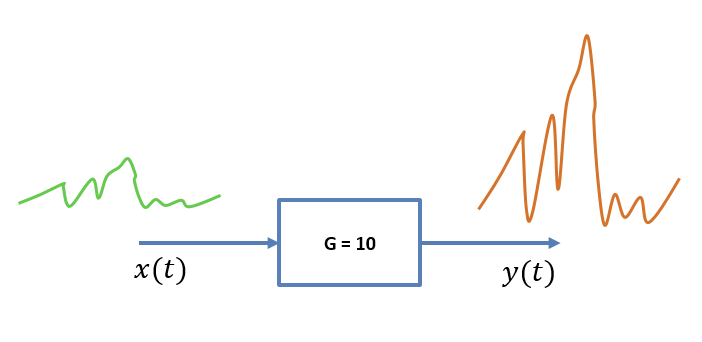
\includegraphics[width=0.6\linewidth]{Figures//Chapter2/Amplifier.png}
    \caption{Amplifier}
    \vspace{-10pt}
    \label{fig:amplifier}
\end{figure}

A time-invariant system is one where a time delay (or shift) in the input sequence causes an equivalent time delay in the system’s output sequence.
\end{block}

\textbf{See Appendix~C of the book "Kalman Filter from the ground up" by Alex Becker for generalized dynamic model derivation for any linear dynamic model.}

\end{frame}

%%%%%%%%%%%%%%%%%%%%%%%%%%%%%%%%%%%%%%%%%

\subsection{Covariance Extrapolation Equation}
\begin{frame}{Covariance Extrapolation Equation}
The general form of the Covariance Extrapolation Equation is given by:
\begin{minipage}{1\linewidth} % Adjust the width as needed
\begin{exampleblock}{}{
\begin{equation*}
\mathbf{P}_{n+1,n} = \mathbf{F}\mathbf{P}_{n,n}\mathbf{F}^T + \mathbf{Q} \tag{2}
\end{equation*}

where:
\begin{itemize}
    \item $\mathbf{P}_{n,n}$ is the squared uncertainty of an estimate (covariance matrix) of the current state.
    \item $\mathbf{P}_{n+1,n}$ is the squared uncertainty of a prediction (covariance matrix) for the next state.
    \item $\mathbf{F}$ is the state transition matrix that we derived in Appendix C (“Modeling linear dynamic systems”).
    \item $\mathbf{Q}$ is the process noise matrix.
\end{itemize}}
\end{exampleblock}
\end{minipage}

\end{frame}
%---------------------------------------------------
\subsubsection{The estimate covariance without process noise}
\begin{frame}{The estimate covariance without process noise}
Assuming $\mathbf{Q}=0$:
$\mathbf{P}_{n+1,n}=\mathbf{F}\mathbf{P}_{n,n}\mathbf{F}^T$

The covariance of a vector \(\mathbf{x}\) is defined as:
\begin{equation*}
{COV}(\mathbf{x}) = \mathbb{E}\left[ (\mathbf{x}-\boldsymbol{\mu}_{\mathbf{x}})(\mathbf{x}-\boldsymbol{\mu}_{\mathbf{x}})^T \right] (\text{vector}~\mathbf{x}~\text{is a system state vector})
\end{equation*}

Therefore, the covariance matrix \(\mathbf{P}_{n,n}\) is:
\begin{equation*}
\mathbf{P}_{n,n} = \mathbb{E}\left[ (\hat{\mathbf{x}}_{n,n} - \boldsymbol{\mu}_{\mathbf{x}_{n,n}})(\hat{\mathbf{x}}_{n,n} - \boldsymbol{\mu}_{\mathbf{x}_{n,n}})^T \right]
\end{equation*}

For the next state, this becomes:
\begin{equation*}
\mathbf{P}_{n+1,n} = \mathbb{E}\left[ (\hat{\mathbf{x}}_{n+1,n} - \boldsymbol{\mu}_{\mathbf{x}_{n+1,n}})(\hat{\mathbf{x}}_{n+1,n} - \boldsymbol{\mu}_{\mathbf{x}_{n+1,n}})^T \right]
\end{equation*}

Following the state extrapolation equation:
\begin{equation*}
\hat{\mathbf{x}}_{n+1,n} = \mathbf{F} \hat{\mathbf{x}}_{n,n} + \mathbf{G}\hat{\mathbf{u}}_{n,n}
\end{equation*}

The update for the covariance matrix can be represented as:
\begin{align*}
\mathbf{P}_{n+1,n} & = \mathbb{E} \left[ (\mathbf{F} \mathbf{\hat{x}}_{n,n} + \mathbf{G}\mathbf{\hat{u}}_{n,n} - \mathbf{F}\mathbf{\mu}_{x,n,n} - \mathbf{G}\mathbf{\hat{u}}_{n,n}) \times (\mathbf{F} \mathbf{\hat{x}}_{n,n} + \mathbf{G}\mathbf{\hat{u}}_{n,n} - \mathbf{F}\mathbf{\mu}_{x,n,n} - \mathbf{G}\mathbf{\hat{u}}_{n,n})^T \right]\\
& = \mathbb{E} \left[ (\mathbf{F} (\mathbf{\hat{x}}_{n,n} - \mathbf{\mu}_{x,n}) ) (\mathbf{F} (\mathbf{\hat{x}}_{n,n} - \mathbf{\mu}_{x,n}) )^T \right]\\
& = \mathbb{E} \left[ (\mathbf{F} (\mathbf{\hat{x}}_{n,n} - \mathbf{\mu}_{x,n}) ) (\mathbf{\hat{x}}_{n,n} - \mathbf{\mu}_{x,n})^T \mathbf{F}^T\right] \quad ((\mathbf{AB})^T = \mathbf{B}^T\mathbf{A}^T)\\
& = \mathbf{F} \mathbb{E} \left[ ( (\mathbf{\hat{x}}_{n,n} - \mathbf{\mu}_{x,n}) ) (\mathbf{\hat{x}}_{n,n} - \mathbf{\mu}_{x,n})^T \right]\mathbf{F}^T \\
&= \mathbf{F}\mathbf{P}_{n,n}\mathbf{F}^T
\end{align*}

\end{frame}
%------------------------------------------
\subsubsection{Constructing the process noise matrix}
\begin{frame}{Constructing the process noise matrix $\mathbf{Q}$}
The system dynamics is described by:
\begin{equation*}
\mathbf{\hat{x}}_{n+1,n} = \mathbf{F}\mathbf{\hat{x}}_{n,n} + \mathbf{G}\mathbf{\hat{u}}_{n,n} + \underset{\text{Process noice}}{\mathbf{w}_n}
\end{equation*}     

In 1D Kalman Filter, the process noise variance is denoted by \textbf{q} while for 3D case by $\mathbf{Q}$. 

The process noise variance has a critical influence on the Kalman
Filter performance. 
\begin{itemize}
    \item Too small $q$ causes a lag error (Example 7).
    \item If the $q$ value is too high, the Kalman Filter follows the measurements (Example 8) and produces noisy estimations.
\end{itemize}

The process noise can be independent between different state variables. In this case, the process noise covariance matrix \( \mathbf{Q} \) is a diagonal matrix:
\begin{equation}
\mathbf{Q} = 
\begin{bmatrix}
q_{11} & 0 & \cdots & 0 \\
0 & q_{22} & \cdots & 0 \\
\vdots & \vdots & \ddots & \vdots \\
0 & 0 & \cdots & q_{kk}
\end{bmatrix}
\tag{8.32}
\end{equation}

The process noise can also be dependent. For example, the constant velocity model assumes zero acceleration (\(a = 0\)). However, a random variance in acceleration (\(\sigma^2_a\)) causes a variance in velocity and position. In this case, the process noise is correlated with the state variables.
\end{frame}


%------------------------------------------
\subsubsection{Discrete Noise Model}
\begin{frame}{Models for the environmental process noise - Discrete Noise}
\begin{columns}
        \column{0.5\textwidth} 
    \textcolor{blue}{There are two models for the environmental process noise; Discrete and Continuous noise model.}
    \begin{figure}
        \centering
        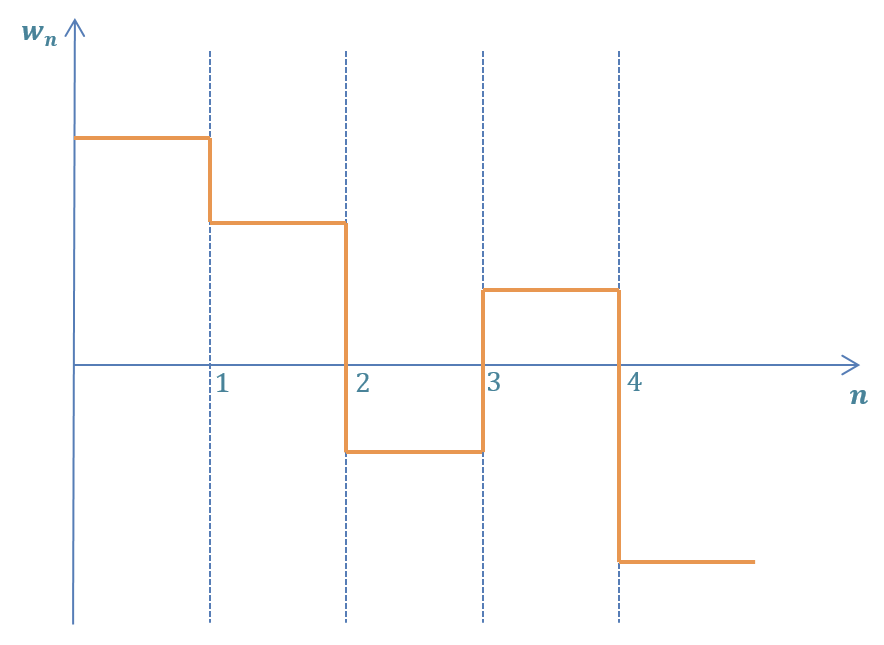
\includegraphics[width=0.6\linewidth]{Figures//Chapter2/DiscreteNoise.png}
        \vspace{-10pt}
        \caption{Discrete Noise}
        \vspace{-10pt}
        \label{fig:DiscreteNoise}
    \end{figure}
    The process noise covariance matrix \(\mathbf{Q}\) for the constant velocity model can be expressed as:
\begin{equation*}
\mathbf{Q} = 
\begin{bmatrix}
V(x) & \text{COV}(x, v) \\
\text{COV}(v, x) & V(v)
\end{bmatrix}
\end{equation*}
where \(V(x)\) and \(V(v)\) represent the position and velocity variance, respectively, and COV(x, v) is the covariance between position and velocity. These terms are expressed in terms of the random acceleration variance \(\sigma_a^2\) of the model.

        \column{0.5\textwidth}
\begin{align*}
V(v) &= \sigma_v^2 = E(v^2) - \mu_v^2\\
 & = E\left((a\Delta t)^2\right) - (\mu_a \Delta t)^2\\
& = \Delta t^2 \left( E(a^2) - \mu_a^2 \right)\\ & = \Delta t^2 \sigma_a^2\\
V(x) &= \sigma_x^2 = E(x^2) - \mu_x^2\\
& = E\left(\left(\frac{1}{2} a \Delta t^2\right)^2\right) - \left(\frac{1}{2} \mu_a \Delta t^2\right)^2\\
& = E\left((a\Delta t)^2\right) - (\mu_a \Delta t)^2\\
& = \Delta t^4 \left( \frac{1}{4} \right) \left( E(a^2) - \mu_a^2 \right)\\ 
& = \Delta t^4 \left( \frac{1}{4} \right) \sigma_a^2\\
\text{COV}(x, v) & = \text{COV}(v, x) = E(xv) - \mu_x\mu_v\\
& = \!\left( E\left( \frac{1}{2} a\Delta t^2 a\Delta t \right) \!-\! \left( \frac{1}{2} \mu_a\Delta t^2 \mu_a\Delta t \right)\! \right)\\ 
& = \frac{\Delta t^3}{2} \left( E(a^2) - \mu_a^2 \right) = \frac{\Delta t^3}{2} \sigma_a^2
\end{align*}
\end{columns}
\end{frame}
%----------------------------------------
\begin{frame}{Discrete Noise-How to construct  $\mathbf{Q}$ matrix}

By substituting the results into $\mathbf{Q}$ matrix:

    $$\mathbf{Q} = \sigma_a^2
\begin{bmatrix}
\frac{\Delta t^4}{4} & \frac{\Delta t^3}{2} \\
\frac{\Delta t^3}{2} & \Delta t^2 \\
\end{bmatrix}$$

There are two methods for a faster construction of the Q matrix
\begin{itemize}
    \item Projection using the state transition matrix (without control input)
    \item Projection using the control matrix (with control input)
\end{itemize}
\end{frame}

%------------------------------------------------
\begin{frame}{Discrete Noise: How to construct  $\mathbf{Q}$ matrix}
\label{DiscreteNoise_ConstructQMatrix}
\begin{columns}
        \column{0.5\textwidth} 
    \textbf{Without Control Input:}
    If the dynamic model doesn’t include a control input,  project the random variance in acceleration $\sigma_a^2$ on the dynamic model using state transition matrix $\mathbf{F}$.
    \begin{itemize}
        \item Let us define a matrix $\mathbf{Q}_a$:
        \[ \mathbf{Q}_a = \begin{bmatrix} 0 & 0 & 0 \\ 0 & 0 & 0 \\ 0 & 0 & 1 \end{bmatrix} \sigma_a^2 \]
        \item The process noise matrix is $\mathbf{Q} = \mathbf{F}\mathbf{Q}_a\mathbf{F}^T$.
        \item For the motion model, $\mathbf{F}$ matrix is:
        \vspace{-10pt}
        \[ \mathbf{F} = \begin{bmatrix} 1 & \Delta t  & \frac{\Delta t^2} {2}\\ 0 & 1 & \Delta t \\ 0 & 0 & 1 \end{bmatrix} \]
    \end{itemize}
    \vspace{-10pt}
    \begin{align*}
    Q \!& =\! \sigma_a^2 \!
    \begin{bmatrix}
    1 & \Delta t & \frac{\Delta t^2}{2} \\
    0 & 1 & \Delta t \\
    0 & 0 & 1 \\
    \end{bmatrix}\!\!\!
    \begin{bmatrix}
    0 & 0 & 0 \\
    0 & 0 & 0 \\
    0 & 0 & 1 \\
    \end{bmatrix}\!\!\!
    \begin{bmatrix}
    1 & 0 & 0 \\
    \Delta t & 1 & 0 \\
    \frac{\Delta t^2}{2} & \Delta t & 1 \\
    \end{bmatrix}\\
    & = \begin{bmatrix}
    \frac{\Delta t^4}{4} & \frac{\Delta t^3}{2} & \frac{\Delta t^2}{2} \\
    \frac{\Delta t^3}{2} & \Delta t^2 & \Delta t \\
    \frac{\Delta t^2}{2} & \Delta t & 1
    \end{bmatrix}
    \end{align*}
        \column{0.5\textwidth}
        \textbf{With Control Input:}
        When the dynamic model includes a control input, we can compute $\mathbf{Q}$ matrix even faster by projecting the random variance in acceleration $\sigma_a^2$ using the control matrix $\mathbf{G}$.

    \begin{itemize}
        \item $\mathbf{Q} = \mathbf{G}\sigma_a^2\mathbf{G}^T$ where $\mathbf{G}$ is the control (or input transition) matrix.
        \item For the motion model, the $\mathbf{G}$ matrix is:
        \[ \mathbf{G} = \begin{bmatrix} \frac{\Delta t^2}{2} \\ \Delta t \end{bmatrix} \]
    \end{itemize}

    \textbf{Resulting $\mathbf{Q}$ matrix:}
    \begin{align*}
        \mathbf{Q} & = \sigma_a^2 \mathbf{G} \mathbf{G}^T\\
        & = \sigma_a^2 \begin{bmatrix} \frac{\Delta t^2}{2} \\ \Delta t \end{bmatrix}\begin{bmatrix} \frac{\Delta t^2}{2} & \Delta t \end{bmatrix}\\
        & = \sigma_a^2 \begin{bmatrix} \frac{\Delta t^4}{4} & \frac{\Delta t^3}{2} \\ \frac{\Delta t^3}{2} & \Delta t^2 \end{bmatrix}
    \end{align*}
\end{columns}
\end{frame}
%---------------------------------------------
\begin{frame}{Continuous Noise: How to construct  $\mathbf{Q}$ matrix }
The continuous model assumes that the noise changes continuously over time.
    \begin{figure}
        \centering
        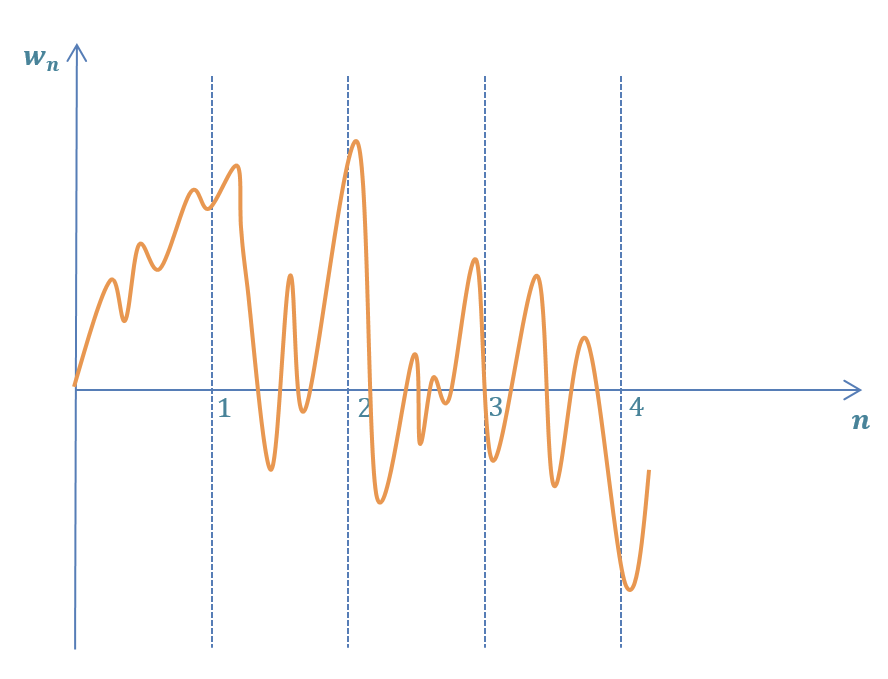
\includegraphics[width=0.4\linewidth]{Figures//Chapter2/ContinuousNoise.png}
        \caption{Continuous Noise}
        \label{fig:ContinuousNoise}
    \end{figure}


To derive the process noise covariance matrix for the continuous model $\mathbf{Q}_c$, we need to integrate the discrete process noise covariance matrix $\mathbf{Q}$ over time.

\[
\mathbf{Q}_{c} = \int_{0}^{\Delta t} \mathbf{Q} dt = \int_{0}^{\Delta t} \sigma_a^2 
\begin{bmatrix}
\frac{t^4}{4} & \frac{t^3}{2} \\
\frac{t^3}{2} & t^2
\end{bmatrix}
dt = \sigma_a^2 
\begin{bmatrix}
\frac{\Delta t^5}{20} & \frac{\Delta t^4}{8} \\
\frac{\Delta t^4}{8} & \frac{\Delta t^3}{3}
\end{bmatrix}
\]
\end{frame}
%---------------------------------------------
\begin{frame}{Selecting Process Noise Variance and Noise Model} 
\begin{block}{Process Noise Variance ($\sigma_a^2$)}
\begin{itemize}
    \item Calculated using stochastic statistics or chosen based on engineering practice.
    \item Depends on target characteristics and model completeness.
    \item For \textbf{maneuvering targets} (e.g., airplanes), $\sigma_a^2$ should be relatively high.
    \item For \textbf{non-maneuvering targets} (e.g., rockets), a smaller $\sigma_a^2$ is appropriate.
    \item Environmental influences like air drag reduce process noise randomness if included in the model.
\end{itemize}
\end{block}

\begin{block}{Choosing the Noise Model}
\begin{itemize}
    \item No definitive answer: recommend trying both discrete and continuous models.
    \item Use \textbf{discrete noise model} when $\Delta t$ is small.
    \item Prefer \textbf{continuous noise model} when $\Delta t$ is high.
    \item Experiment to see which model performs better with your Kalman Filter.
\end{itemize}
\end{block}
\end{frame}

%-------------------------------------------------------
\subsection{Auxiliary Equations}
\subsubsection{Measurement Equation}
\begin{frame}{Measurement Equation}
In 1D KF, measurement denoted by $z_n$
\begin{itemize}
    \item Represented the true system state plus random measurement noise $v_n$.
\end{itemize}

Measurement Noise Variance ($r_n$):
\begin{itemize}
    \item Can be \textbf{constant} for all measurements (e.g., scales with a precision of 0.5 kg).
    \item May \textbf{vary} for each measurement (e.g., thermometer with 0.5\% precision).
    \item In variable cases, the noise variance depends on the measured quantity (e.g., temperature).
\end{itemize}

\begin{minipage}{1\linewidth} 
\begin{exampleblock}{}{
The Measurement Equation is given by:
\begin{equation*}
\mathbf{z}_n = \mathbf{H}\mathbf{x}_n + \mathbf{v}_n
\end{equation*}

where:
\begin{itemize}
    \item $\mathbf{z}_n$ is a measurement vector.
    \item $\mathbf{x}_n$ is a true system state (hidden state).
    \item $\mathbf{v}_n$ is a random noise vector.
    \item $\mathbf{H}$ is an observation matrix.
\end{itemize}}
\end{exampleblock}
\end{minipage}

\end{frame}
%------------------------------------------------------------
\begin{frame}{The Observation Matrix}

In many scenarios, the measured value is not the direct system state we are interested in. For instance, a digital electric thermometer measures an electric current, which needs to be translated to temperature -- the actual system state of interest.

\vspace{5pt}
The observation matrix $\mathbf{H}$ serves the crucial function of transforming the system state (input) into the measurement (output) through linear transformations. This process ensures that the Kalman Filter can work with measurements that represent the system states accurately.

\vspace{5pt}
\textbf{Scaling:} A range meter sends a signal toward a destination and receives a reflected echo. The
measurement is the time delay between the transmission and reception of the signal. The system state is the range.

In this case, we need to perform a scaling:
\begin{equation*}
z_n = \begin{bmatrix} \frac{2}{c} \end{bmatrix} x_n + v_n
\end{equation*}
\begin{equation*}
H = \begin{bmatrix} \frac{2}{c} \end{bmatrix}
\end{equation*}

where:
\begin{itemize}
    \item \(c\) is the speed of light.
    \item \(x_n\) is the range.
    \item \(z_n\) is the measured time delay.
\end{itemize}

\end{frame}
%------------------------------------------------------------
\begin{frame}{The Observation Matrix}
\textbf{State selection:} Sometimes certain states are measured while others are not. For example, the first,
third, and fifth states of a 5D state vector are measurable, while the second and fourth states are not measurable:
$$z_n = \mathbf{H}\mathbf{x}_n + \mathbf{v}_n = 
\begin{bmatrix}
1 & 0 & 0 & 0 & 0 \\
0 & 0 & 1 & 0 & 0 \\
0 & 0 & 0 & 0 & 1 \\
\end{bmatrix}
\begin{bmatrix}
x_1 \\
x_2 \\
x_3 \\
x_4 \\
x_5 \\
\end{bmatrix}
+ \mathbf{v}_n = 
\begin{bmatrix}
x_1 \\
x_3 \\
x_5 \\
\end{bmatrix}
+ \mathbf{v}_n$$

\textbf{Combination of states:} Sometimes some combination of states can be measured instead of each separate
state. For example, maybe the lengths of the sides of a triangle are the states, and only the total perimeter can be measured:

$$z_n = \mathbf{H}\mathbf{x}_n + \mathbf{v}_n = 
\begin{bmatrix}
1 & 1 & 1 \\
\end{bmatrix}
\begin{bmatrix}
x_1 \\
x_2 \\
x_3 \\
\end{bmatrix}
+ \mathbf{v}_n = (x_1 + x_2 + x_3) + \mathbf{v}_n$$

\end{frame}
%------------------------------------------------------------
\subsubsection{Covariance Equations}
\begin{frame}{Covariance Equations}
    The terms $\mathbf{w}$ and $\mathbf{v}$, which correspond to the process and measurement noise, do not typically appear directly in the calculations since they are unknown. Instead, these terms are used to model the uncertainty (or noise) in the equations themselves.

    \vspace{5pt}
    All covariance equations are covariance matrices in the form of:

    $$E(\mathbf{e}\mathbf{e}^T)$$

    i.e., an expectation of a squared error.
\begin{itemize}
    \item \textbf{Measurement uncertainty:} $$\mathbf{R}_n = E(\mathbf{v}_n\mathbf{v}_n^T)$$

    \item \textbf{Process noise uncertainty:} $$\mathbf{Q}_n = E(\mathbf{w}\mathbf{w}^T)$$

    \item \textbf{Estimation uncertainty:} $$\mathbf{P}_n = E(\mathbf{e}_n\mathbf{e}_n^T) = E \left((x_n - \hat{x}_{n,n})(x_n - \hat{x}_{n,n})^T\right)$$
\end{itemize}
    
\end{frame}

%------------------------------------------------------------

\subsection{State Update Equation}
\begin{frame}{State Update Equation}
\begin{minipage}{1\linewidth} 
\begin{exampleblock}{}{
The State Update Equation is given by:
\begin{equation*}
\hat{\mathbf{x}}_{n,n} = \hat{\mathbf{x}}_{n,n-1} + \mathbf{K}_n(\mathbf{z}_n - \mathbf{H}\hat{\mathbf{x}}_{n,n-1}) \tag{3}
\end{equation*}

where:
\begin{itemize}
    \item $\hat{\mathbf{x}}_{n,n}$ is an estimated system state vector at time step \(n\).
    \item $\hat{\mathbf{x}}_{n,n-1}$ is a predicted system state vector at time step \(n - 1\).
    \item $\mathbf{K}_n$ is the Kalman Gain.
    \item $\mathbf{z}_n$ is a measurement.
    \item $\mathbf{H}$ is an observation matrix.
\end{itemize}}
\end{exampleblock}
\end{minipage}

\end{frame}


%------------------------------------------------------------
\subsection{Covariance Update Equation}
\begin{frame}{Covariance Update Equation}
\begin{minipage}{1\linewidth} 
\begin{exampleblock}{}{
The Covariance Update Equation is given by:
\begin{equation*}
\mathbf{P}_{n,n} = (\mathbf{I} - \mathbf{K}_n\mathbf{H})\mathbf{P}_{n,n-1}(\mathbf{I} - \mathbf{K}_n\mathbf{H})^T + \mathbf{K}_n\mathbf{R}_n\mathbf{K}_n^T \tag{4}
\end{equation*}

where:
\begin{itemize}
    \item $\mathbf{P}_{n,n}$ is the covariance matrix of the current state estimation.
    \item $\mathbf{P}_{n,n-1}$ is the prior estimate covariance matrix of the current state (predicted at the previous state).
    \item $\mathbf{K}_n$ is the Kalman Gain.
    \item $\mathbf{H}$ is the observation matrix.
    \item $\mathbf{R}_n$ is the measurement noise covariance matrix.
    \item $\mathbf{I}$ is an Identity Matrix (the \(n \times n\) square matrix with ones on the main diagonal and zeros elsewhere).
\end{itemize}}
\end{exampleblock}
\end{minipage}

\textbf{See derivation in the book.}
\end{frame}
%------------------------------------------------------------
\begin{frame}{Simplified Covariance Update Equation}
A simplified form of the Covariance Update Equation is:
\begin{equation*}
\mathbf{P}_{n,n} = (\mathbf{I} - \mathbf{K}_n\mathbf{H})\mathbf{P}_{n,n-1}
\end{equation*}

\textcolor{red}{This equation is much more elegant and easier to remember and it performs well in many cases. However, a minor error in computing the Kalman Gain (due to round-off) can lead to huge computation errors. The subtraction $(\mathbf{I} - \mathbf{K}_n\mathbf{H})$ can lead to nonsymmetric matrices due to floating-point errors. This equation is numerically unstable!}
\end{frame}

%------------------------------------------------------------
\subsection{The Kalman Gain}
\begin{frame}{The Kalman Gain}
\begin{minipage}{1\linewidth} 
\begin{exampleblock}{}{
The Kalman Gain Equation is given by:
\begin{equation*}
\mathbf{K}_n = \mathbf{P}_{n,n-1}\mathbf{H}^T \left( \mathbf{H}\mathbf{P}_{n,n-1}\mathbf{H}^T + \mathbf{R}_n \right)^{-1} \tag{5}
\end{equation*}

Where:
\begin{itemize}
    \item $\mathbf{K}_n$ is the Kalman Gain.
    \item $\mathbf{P}_{n,n-1}$ is the prior estimate covariance matrix of the current state (predicted at the previous step).
    \item $\mathbf{H}$ is the observation matrix.
    \item $\mathbf{R}_n$ is the measurement noise covariance matrix.
\end{itemize}}
\end{exampleblock}
\end{minipage}

\textbf{See derivation in the book.}
\end{frame}

%----------------------------------
\begin{frame}{Summary}
The Kalman Filter operates in a "predict-correct"
loop:
\begin{columns}
        \column{0.4\textwidth} 
        \begin{figure}
            \centering
            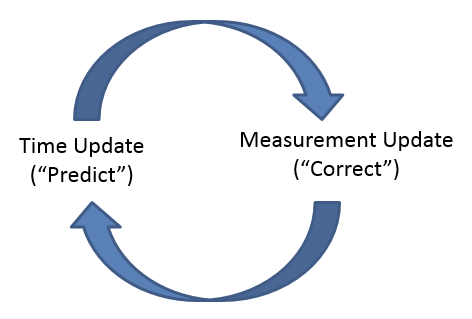
\includegraphics[width=0.6\linewidth]{Figures//Chapter2/Predict_Update_KF.png}
            \caption{Predict Update Diagram}
            \label{fig:PredictUpdateDiagram}
        \end{figure}
        \column{0.6\textwidth}
        \begin{figure}
            \centering
            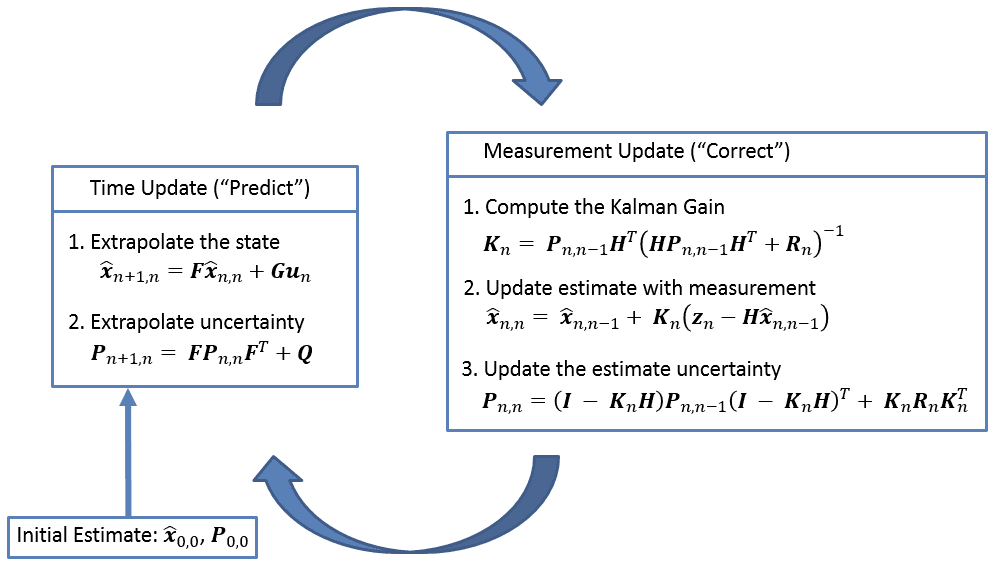
\includegraphics[width=1\linewidth]{Figures//Chapter2/KF_Diagram.png}
            \caption{Kalman Filter diagram}
            \label{fig:KF_Diagram}
        \end{figure}
\end{columns}
\begin{itemize}
    \item Once initialized, the Kalman Filter \textcolor{blue}{predicts} the system state at the next step. It also provides the uncertainty of the prediction.
    \item Once the measurement is received, the Kalman Filter \textcolor{blue}{updates} (or \textcolor{blue}{corrects}) the prediction and the uncertainty of the current state. As well the Kalman Filter predicts the following states, and so on. The following diagram provides a complete picture of the Kalman Filter operation.
\end{itemize}
    
\end{frame}

%----------------------------------
\begin{frame}{Summary}
\vspace{-7pt}
\begin{figure}
    \centering
    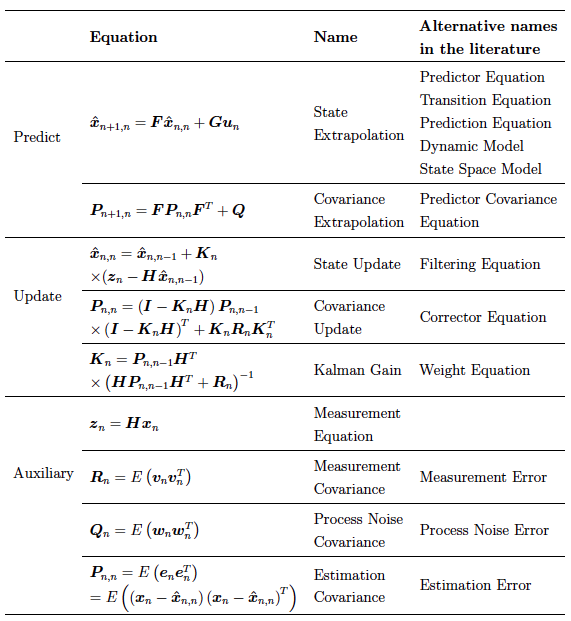
\includegraphics[width=0.55\linewidth]{Figures//Chapter2/KF Equations.png}
    \caption{KF Equations}
    \vspace{-15pt}
    \label{fig:KF_Equations}
\end{figure}
\end{frame}